\section{Resultados y discusión}

\subsection{Análisis Cuantitativo}
\subsubsection{Tiempo de Cómputo}
\textbf{Objetivo}:
El objetivo de este experimento consiste en determinar el tiempo de cómputo de ambos métodos y compararlos en función del tamaño de la entrada. Para lograrlo variamos la cantidad de filas que tomamos de la imagen (la altura) dejando el ancho constante. Iteramos 100 veces comenzando desde la fila 10 y aumentamos en cada paso en dos la cantida de filas a considerar.\\
Para implementarlo se utilizó la función clock de libreria standard de C++.\\

\textbf{Hipótesis:}

Eliminación Gaussiana tiene una complejidad asintótica lineal en nuestra implementación.

\textbf{Resultados y discusión:}

\begin{figure}[H]	
	\centering
	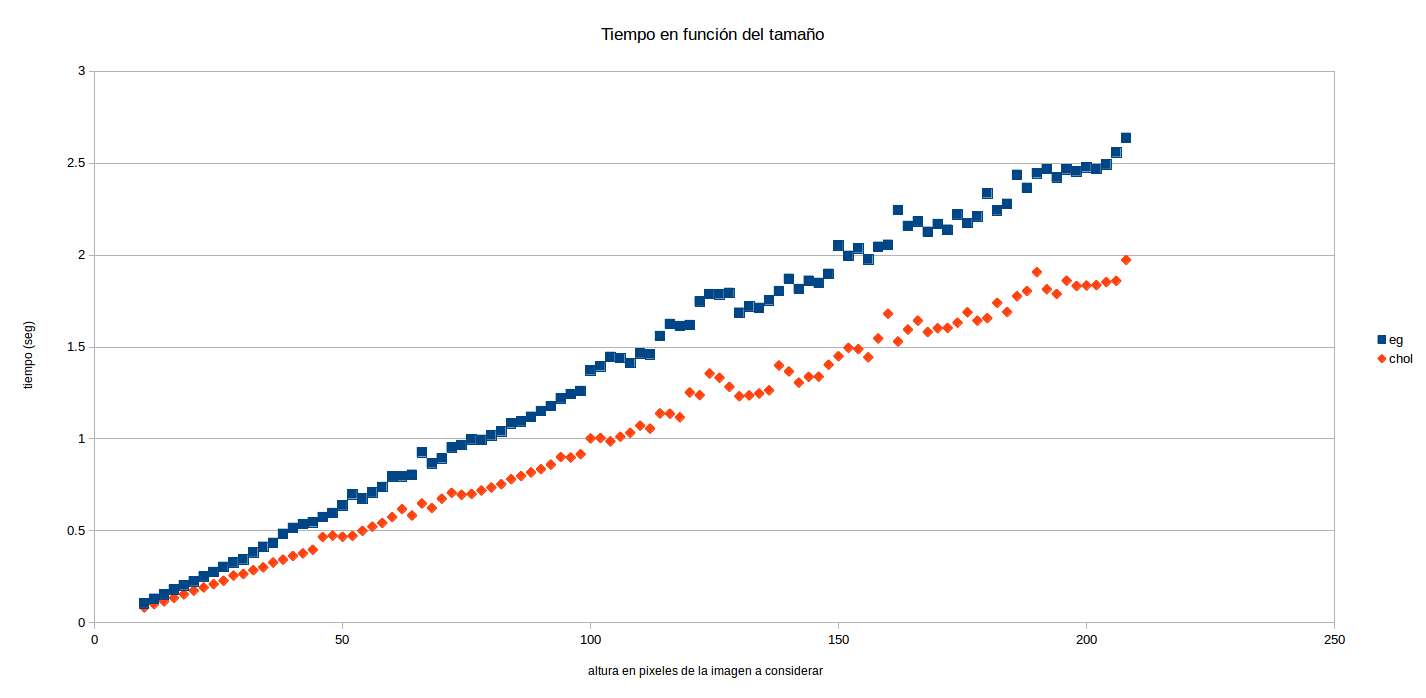
\includegraphics[width=1\linewidth]{img/tiempos.png}
	\caption{Normales buda con direcciones de luz 0 , 3 y 4}
    \label{fig:resultado}
\end{figure}

Se observa que el método de eliminación Gaussiana requiere de mayor número de operaciones para finalizar su cálculo, estado la factorización de Cholesky levemente debajo de lo demanda el primero. \\
El tiempo parece crecer linealmente en función del tamaño de la entrada. Es por eso que lo normalizamos dividiendo por la cantidad de filas a considerar, obteniendo el siguiente resultado:

\begin{figure}[H]	
	\centering
	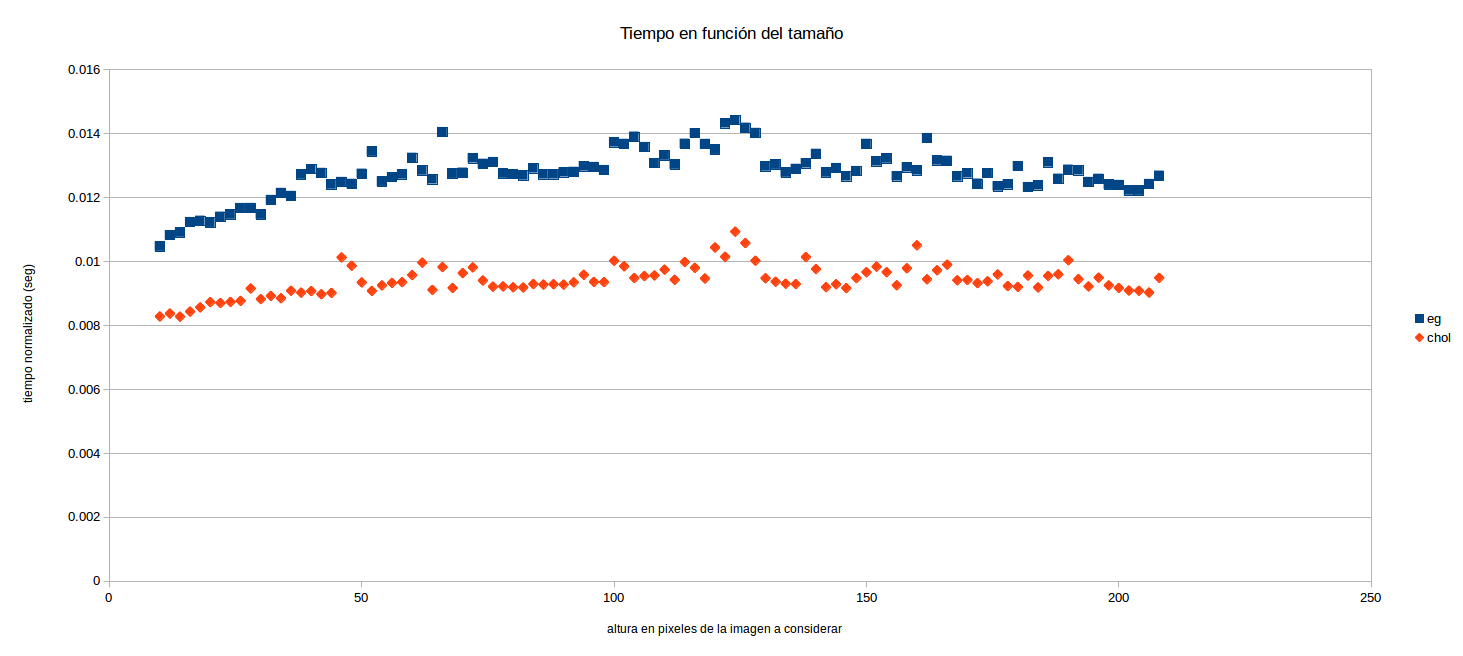
\includegraphics[width=1\linewidth]{img/tiemposnormalizados.png}
	\caption{Normales buda con direcciones de luz 0 , 3 y 4}
    \label{fig:resultado}
\end{figure}

La función se aproxima a una constante por lo que el tiempo que demanda calcular las profundidades utilizando cualquiera de los dos métodos parece tender a una función lineal en la cantidad de píxeles tomados.

\subsection{Análisis Cualitativo}
\subsubsection{Comparación de direcciones de iluminación obtenidas por calibración}
\textbf{Objetivo}:
El objetivo de este experimento es 


\textbf{Hipótesis:}

\textbf{Resultados y discusión:}

calibracion propia
\begin{center}

    \begin{tabular}{ | l | l | l | l |}
    \hline
    Imagen & x & y & z \\ \hline
    0 & 0.506912 & 0.43318 & 0.745248 \\ \hline
    1 & 0.170507 & 0.0230415 & 0.985087 \\ \hline
    2 & -0.00329164 & 0.349572 & 0.936904 \\ \hline
    3 & -0.0230415 & 0.290323 & 0.956651 \\ \hline
    4 & -0.142857 & 0.317972 & 0.937276 \\ \hline
    5 & -0.0230415 & 0.290323 & 0.956651 \\ \hline
    6 & 0.170507 & 0.0322581 & 0.984828 \\ \hline
    7 & 0.0691244 & 0.262673 & 0.962406 \\ \hline
    8 & 0.170507 & 0.0322581 & 0.984828 \\ \hline 
    9 & 0.16129 & 0.0322581 & 0.98638 \\ \hline
    10 & 0.164363 & 0.0291859 & 0.985968 \\ \hline
    11 & -0.0175115 & 0.306912 & 0.951577 \\ \hline
    \hline
    \end{tabular}
\end{center}

calibraicon cátedra
\begin{center}
    \begin{tabular}{ | l | l | l | l |}
    \hline
    Imagen & x & y & z \\ \hline
    0 & 0.403259 &  0.480808 & 0.778592 \\ \hline
    1 & 0.0982272 & 0.163712 & 0.981606 \\ \hline
    2 & -0.0654826 & 0.180077 & 0.98147 \\ \hline
    3 & -0.127999 & 0.431998 & 0.892745 \\ \hline
    4 & -0.328606 & 0.485085 & 0.810377\\ \hline
    5 & -0.110339 & 0.53593 & 0.837021 \\ \hline
    6 & 0.239071 & 0.41439 & 0.878138 \\ \hline
    7 & 0.0642302 & 0.417497 & 0.906406 \\ \hline
    8 & 0.12931 & 0.339438 & 0.931698 \\ \hline 
    9 & 0.0323953 & 0.340151 & 0.939813 \\ \hline
    10 & 0.0985318 & 0.0492659 & 0.993914\\ \hline
    11 & -0.16119 & 0.354617 & 0.921013 \\ \hline
    \hline
    \end{tabular}
\end{center}

Se asemejan bastante las calibraciones.

\subsubsection{Efecto de la calibración en el resto de las etapas}
\textbf{Objetivo}:
El objetivo de este experimento es 
\\
\textbf{Hipótesis:}

\textbf{Resultados y discusión:}


\subsubsection{Impacto de las direcciones de iluminación en el cálculo de las normales}
\textbf{Objetivo}:
El objetivo de este experimento es determinar de qué manera la elección de las direcciones de iluminación impacta en el cálculo de las normales. 


\textbf{Hipótesis:}


\textbf{Resultados y discusión:}


%\begin{figure}[H]
%    \center
%    \includegraphics[width=0.8\textwidth]{img/budada034.png}
%\end{figure}


En este caso tomamos a buda con las direcciones de Luces 0,3 y 4.

\begin{figure}[H]	
	\centering
	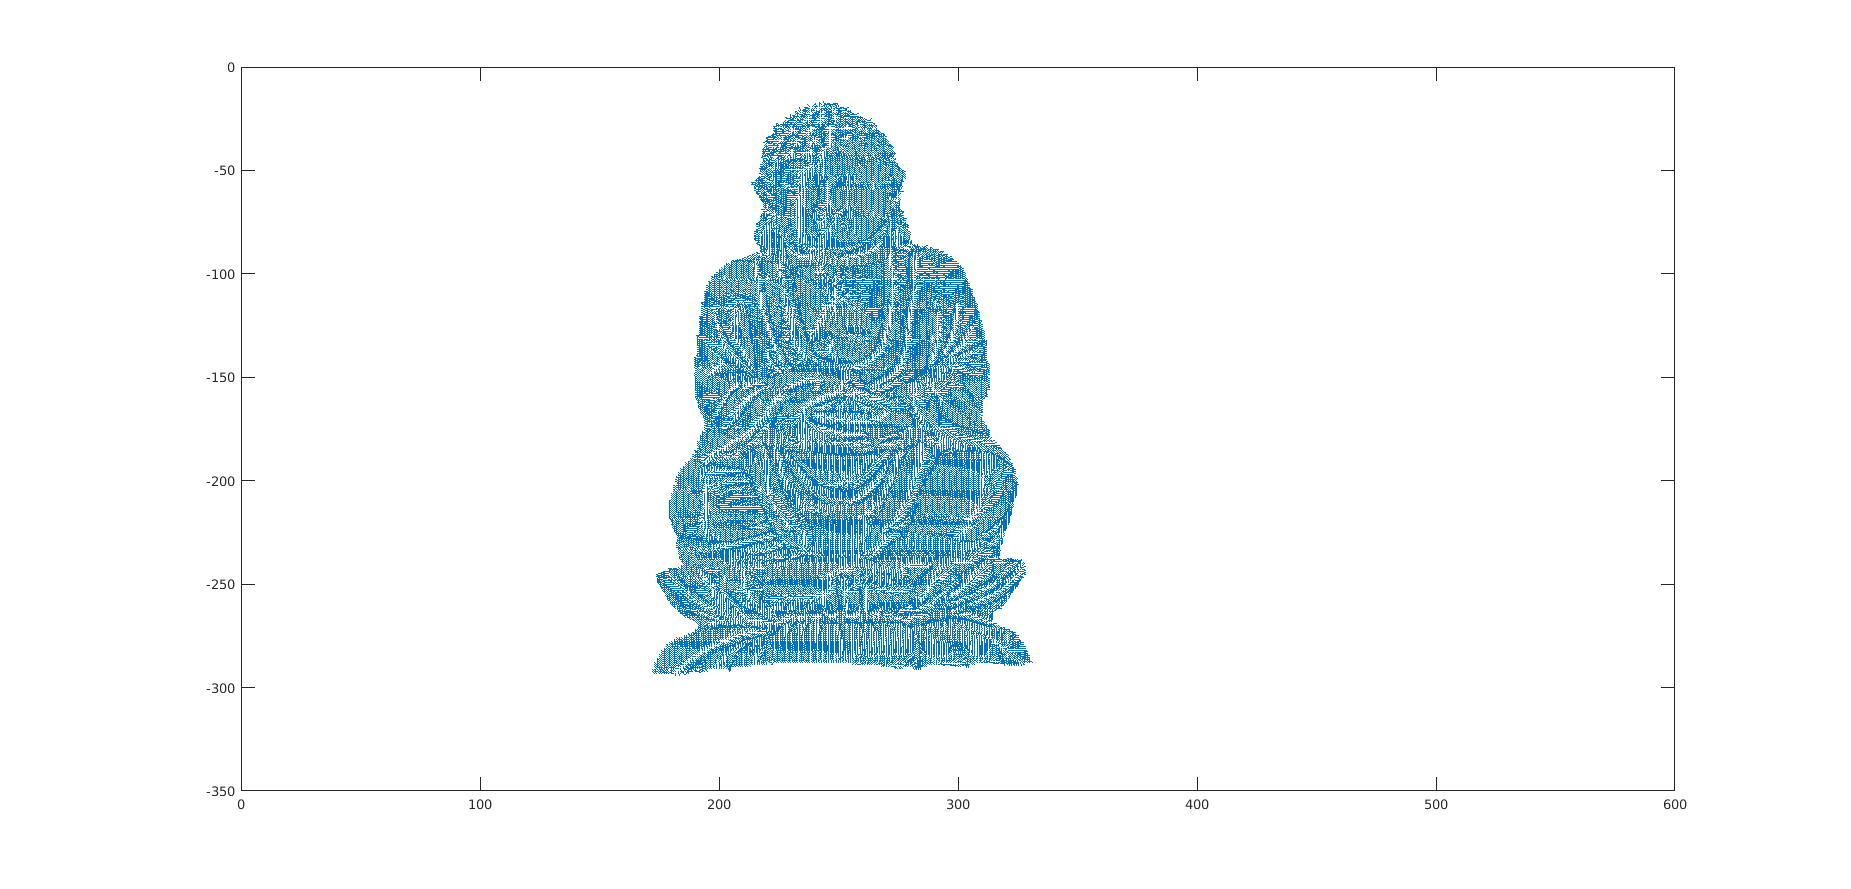
\includegraphics[width=1\linewidth]{img/buda034normales.png}
	\caption{Normales buda con direcciones de luz 0 , 3 y 4}
    \label{fig:resultado}
\end{figure}

\begin{figure}[H]	
	\centering
	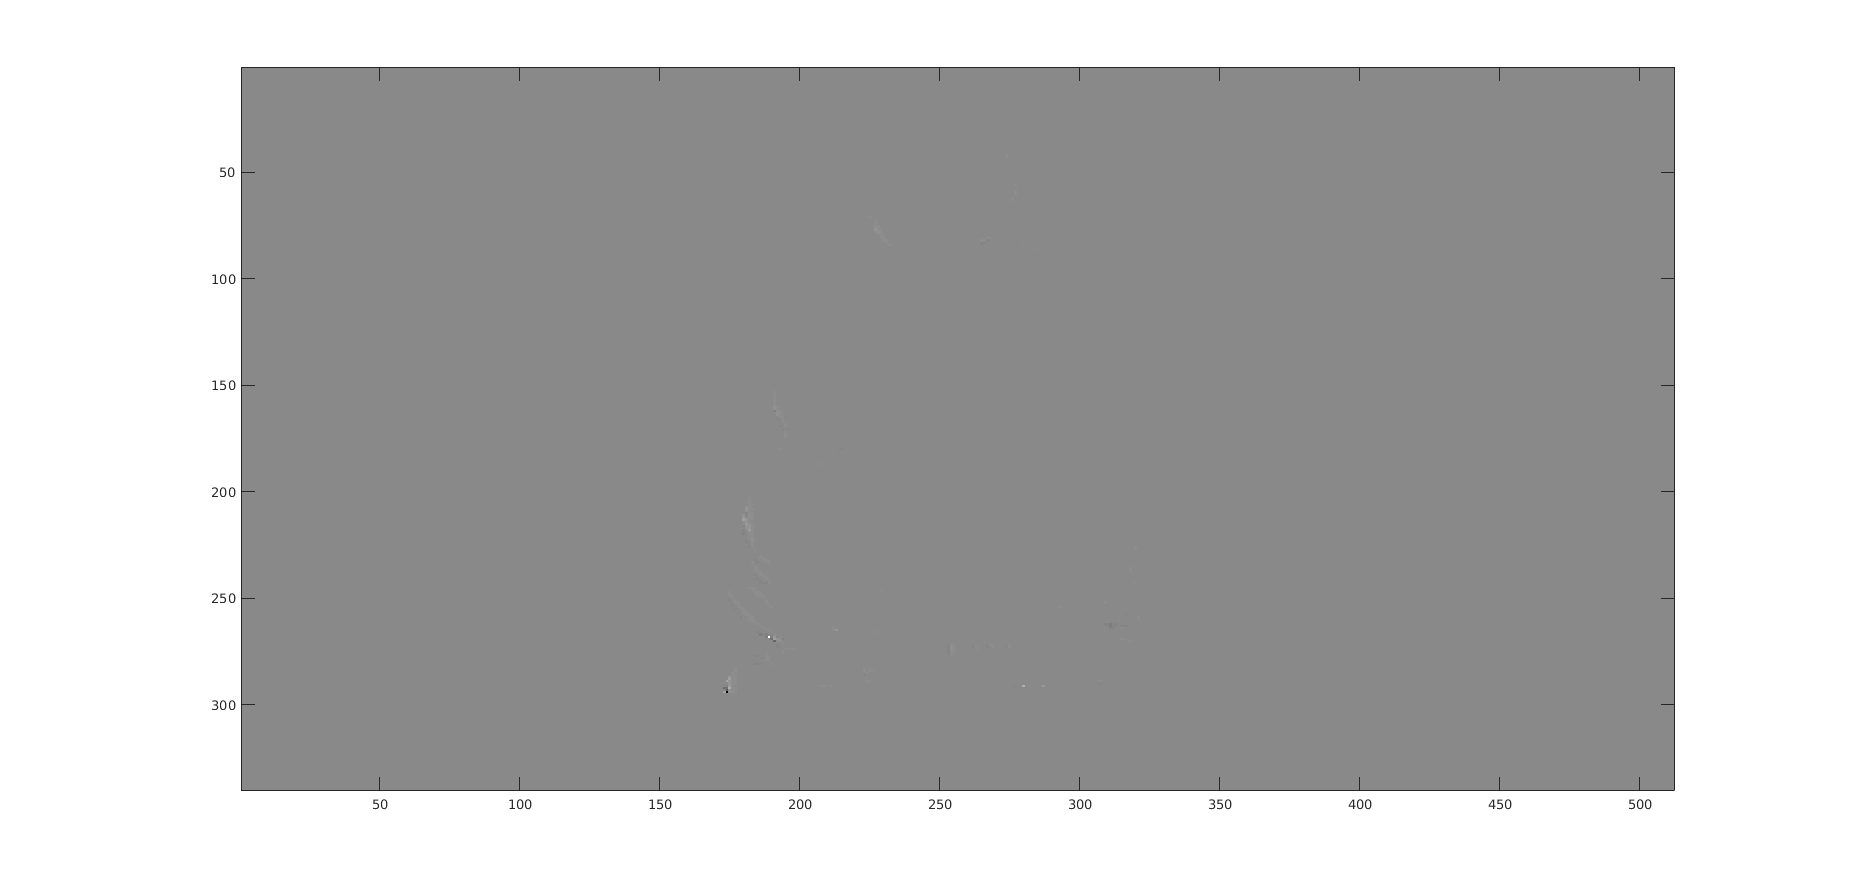
\includegraphics[width=1\linewidth]{img/buda034depth.png}
	\caption{Normales buda con direcciones de luz 0 , 3 y 4}
    \label{fig:resultado}
\end{figure}

\begin{figure}[H]	
	\centering
	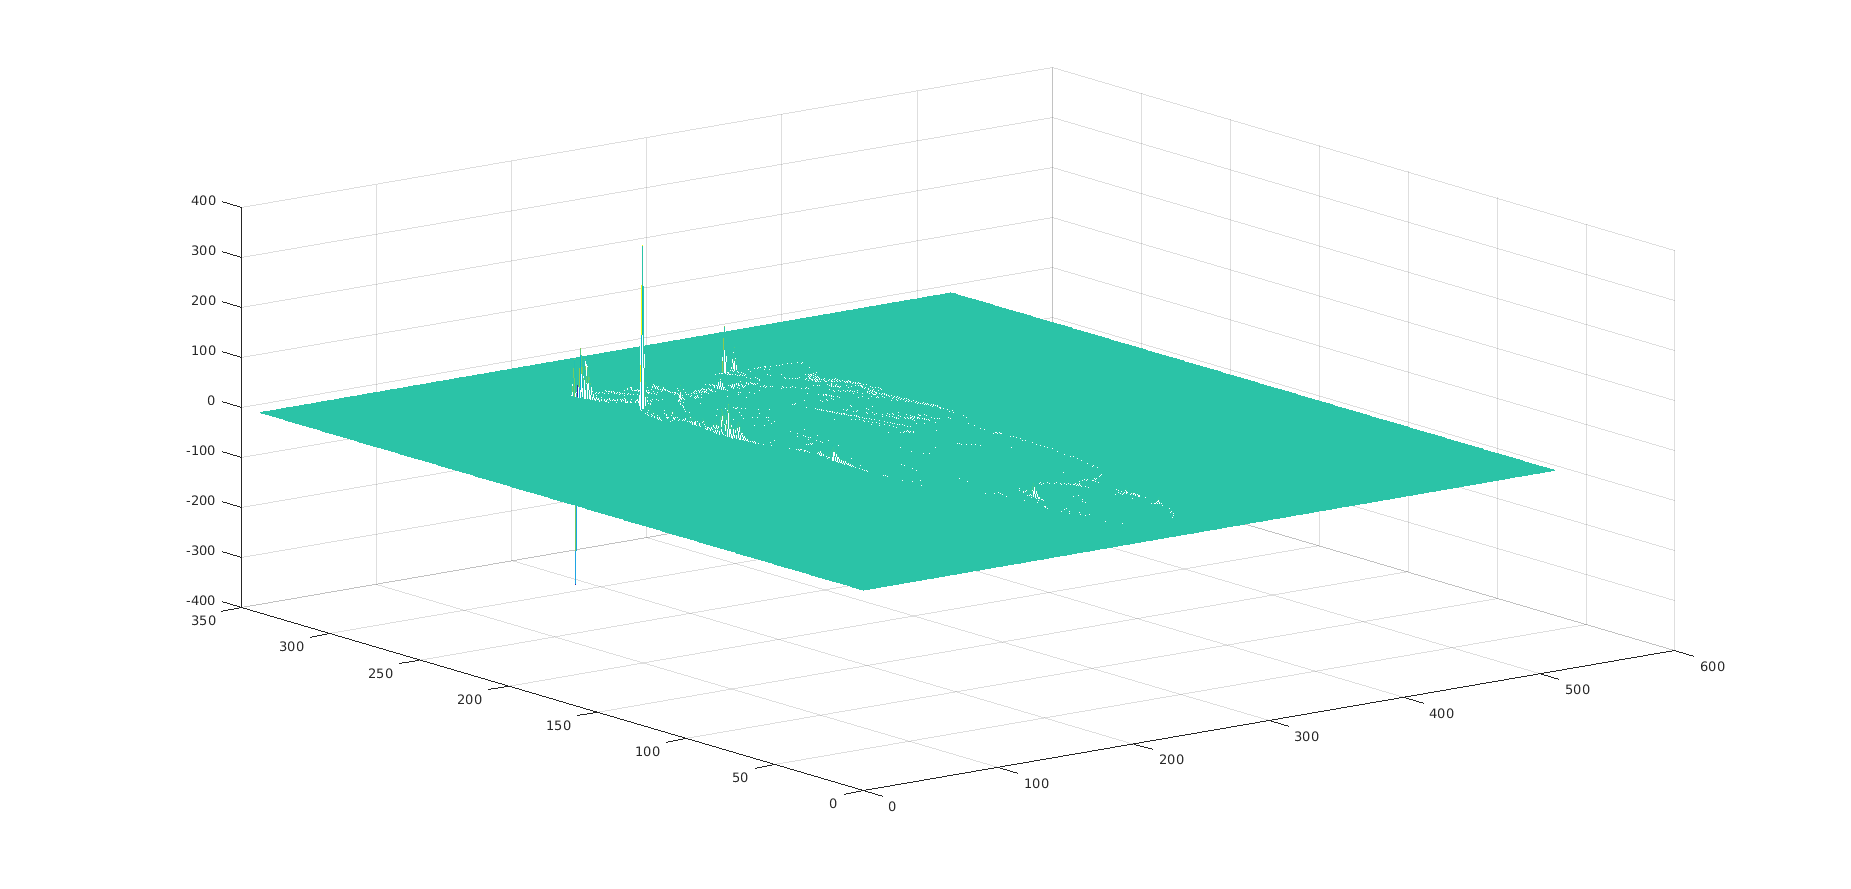
\includegraphics[width=1\linewidth]{img/buda034modelo.png}
	\caption{Normales buda con direcciones de luz 0 , 3 y 4}
    \label{fig:resultado}
\end{figure}